\documentclass[lualatex,aspectratio=169]{beamer}
\usepackage[T1]{fontenc}
\usepackage{luatexja}
\usepackage[deluxe]{luatexja-preset} 
\usepackage{amsmath}
\usepackage{tikz}
\usepackage{listings}
\lstset{
  basicstyle=\footnotesize\ttfamily,
  keywordstyle=\color{blue},
  language=[LaTeX]TeX,
  breaklines=true,
  showstringspaces=false,
}
\setmainjfont{Hiragino Kaku Gothic ProN}

\usetheme[progressbar=none]{metropolis}

\usepackage{xcolor}
\definecolor{hf-orange}{HTML}{FFA700}
\definecolor{hf-orange-dark}{HTML}{FF882B}
\definecolor{hf-blue}{HTML}{4884DA}
\definecolor{hf-blue-dark}{HTML}{4D6BD5}
\definecolor{hf-orange-gradient-left}{HTML}{FF882B}
\definecolor{hf-orange-gradient-right}{HTML}{FFE721}
\definecolor{hf-blue-gradient-left}{HTML}{48D2E6}
\definecolor{hf-blue-gradient-right}{HTML}{4D6BD5}

\setbeamertemplate{footline}{%
  \begin{tikzpicture}[remember picture, overlay]
    % left half of the bar
    \shade[left color=hf-orange-gradient-left, right color=hf-orange-gradient-right]
      (current page.south west) rectangle ([yshift=0.5mm]current page.south);

    % right half of the bar
    \shade[left color=hf-blue-gradient-left, right color=hf-blue-gradient-right]
      (current page.south) rectangle ([yshift=0.5mm]current page.south east);

    % slide number
    \node[
      anchor=east,
      xshift=-5mm,
      yshift=5mm,
      font=\sffamily\color{mDarkTeal}
    ]
    at (current page.south east)
    {\insertframenumber};
  \end{tikzpicture}%
}

\setbeamertemplate{title separator}{
  
\begin{tikzpicture}
    % Left half of the bar
    \shade[left color=hf-orange-gradient-left, right color=hf-orange-gradient-right]
      (0,0) rectangle (0.5\textwidth, 0.25mm);
    % Right half of the bar
    \shade[left color=hf-blue-gradient-left, right color=hf-blue-gradient-right]
      (0.5\textwidth,0) rectangle (\textwidth, 0.25mm);
  \end{tikzpicture}
  \vskip1em % Adds a little vertical space after the separator
}

\setbeamertemplate{section page}{
  \begin{center}
    \usebeamerfont{section title}
    \usebeamercolor[fg]{section title}
    \insertsection
    \par % Creates a new paragraph for spacing
    
\begin{tikzpicture}
      % Left half of the bar
      \shade[left color=hf-orange-gradient-left, right color=hf-orange-gradient-right]
        (0,0) rectangle (0.5\textwidth, 0.25mm);
      % Right half of the bar
      \shade[left color=hf-blue-gradient-left, right color=hf-blue-gradient-right]
        (0.5\textwidth,0) rectangle (\textwidth, 0.25mm);
    \end{tikzpicture}
  \end{center}
}

\setbeamercolor{frametitle}{fg=mDarkTeal, bg=black!2}
\setbeamertemplate{frametitle}{
  \nointerlineskip%
  \begin{tikzpicture}
    % use the full paper width and a height of 5ex
    \useasboundingbox (0,0) rectangle (\paperwidth, 5ex);

    % background for the entire header
    \fill[black!2] (0,0) rectangle (\paperwidth, 5ex);

    % thin gradient bar on the left (top to bottom)
    \shade[top color=hf-orange-gradient-left, bottom color=hf-orange-gradient-right] (0,0) rectangle (1.5mm, 5ex);

    % frame title text (mDarkTeal on black!2)
    \node[
      anchor=west,      % align text to the left
      inner xsep=1em,     % add padding between bar and text
      text=mDarkTeal
    ] at (2mm, 2.5ex) { % position the node
      \usebeamerfont{frametitle}\insertframetitle
    };
  \end{tikzpicture}%
}

\title{ウェブ上の学術論文}
\subtitle{PDFの代替になれるか / アクセシビリティーの観点 / 先進的取組の事例}
\author{tarek（タレク）}
\institute{株式会社Helpfeel}
\date{}

\begin{document}

\begin{frame}[plain]
  \titlepage
\end{frame}

% \begin{frame}[t]{目次}
%   \tableofcontents
% \end{frame}

% \section{自己紹介}

\begin{frame}[t]{学術論文}
    \begin{figure}
        \begin{overprint}
            \onslide<1>\begin{center}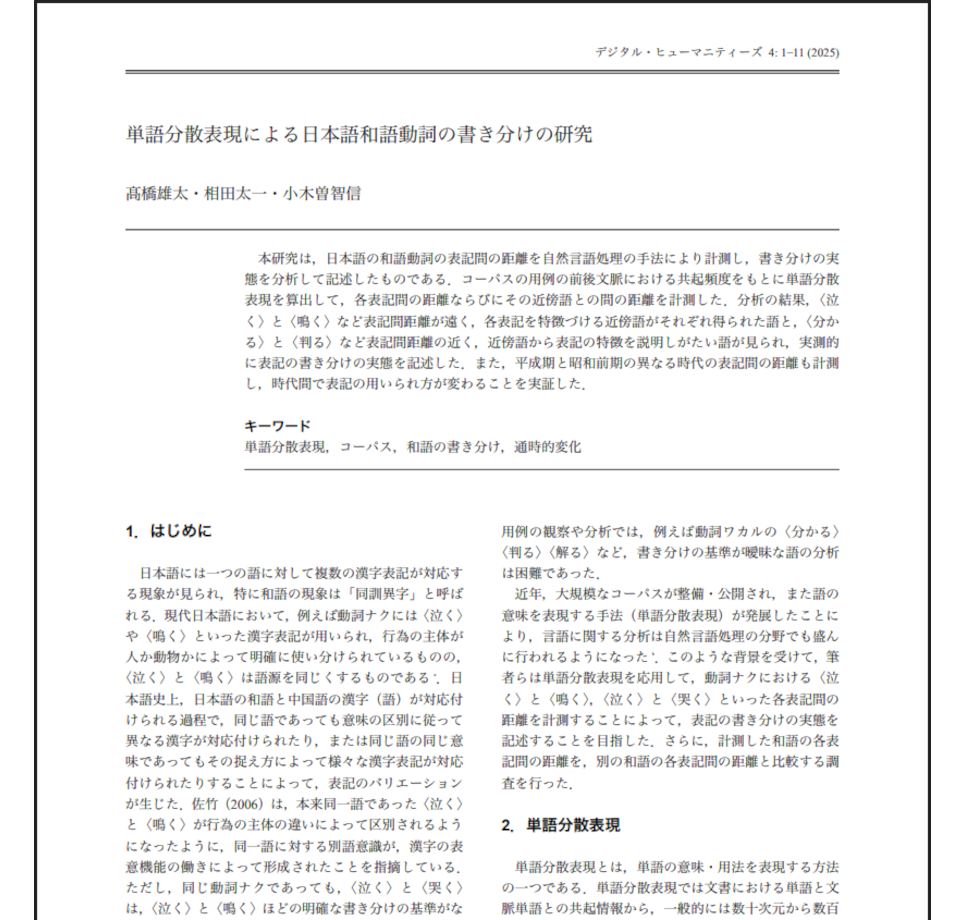
\includegraphics[height=0.80\textheight]{./img/ja_paper_pdf_1.png}\end{center}
            \onslide<2>\begin{center}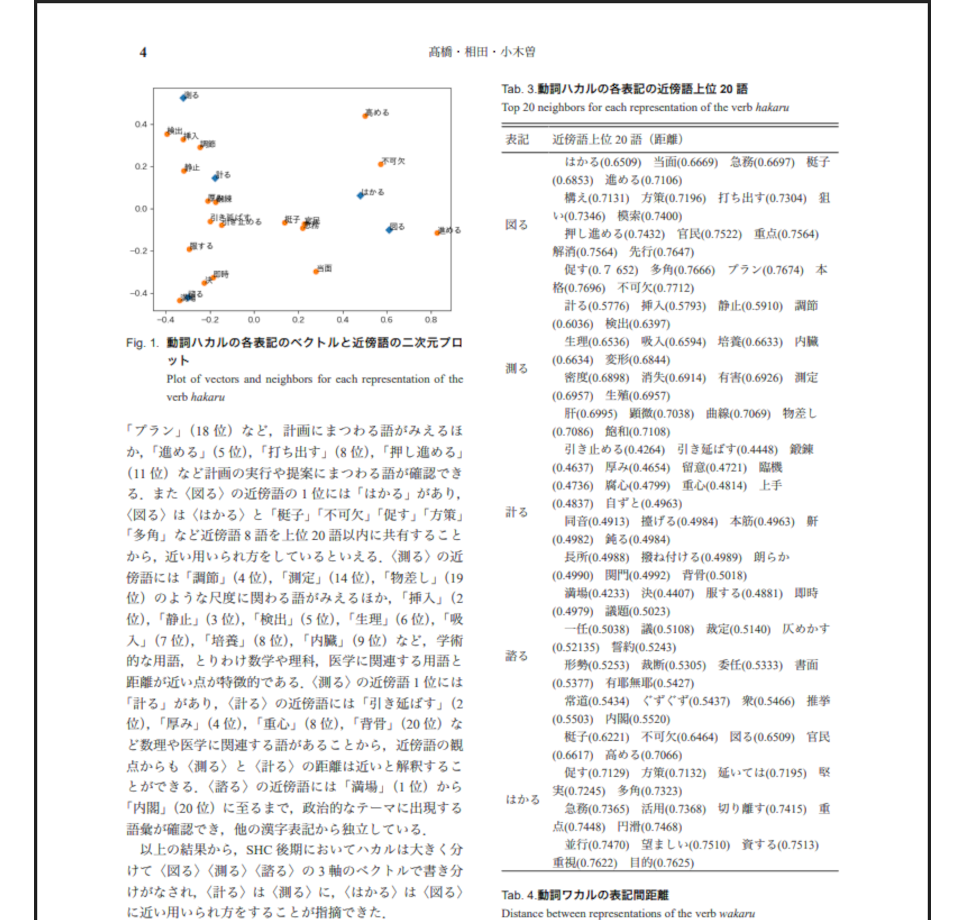
\includegraphics[height=0.80\textheight]{./img/ja_paper_pdf_2.png}\end{center}
            \onslide<3>\begin{center}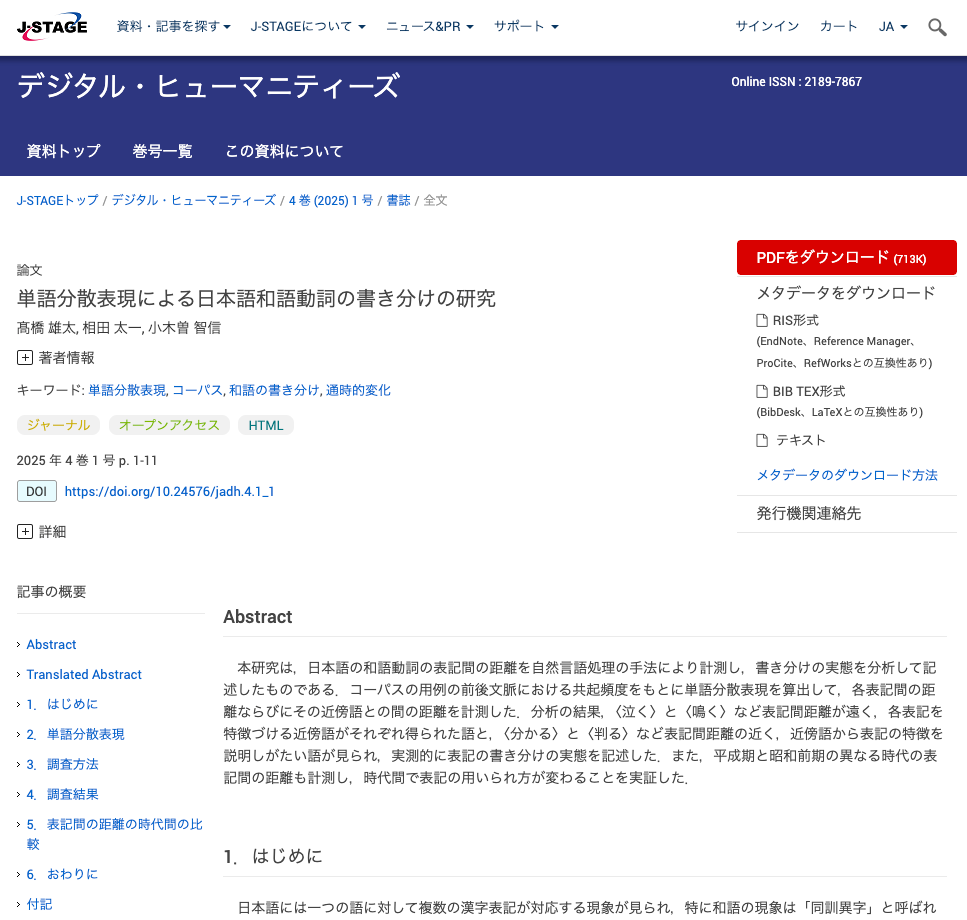
\includegraphics[height=0.80\textheight]{./img/ja_paper_web_1.png}\end{center}
            \onslide<4>\begin{center}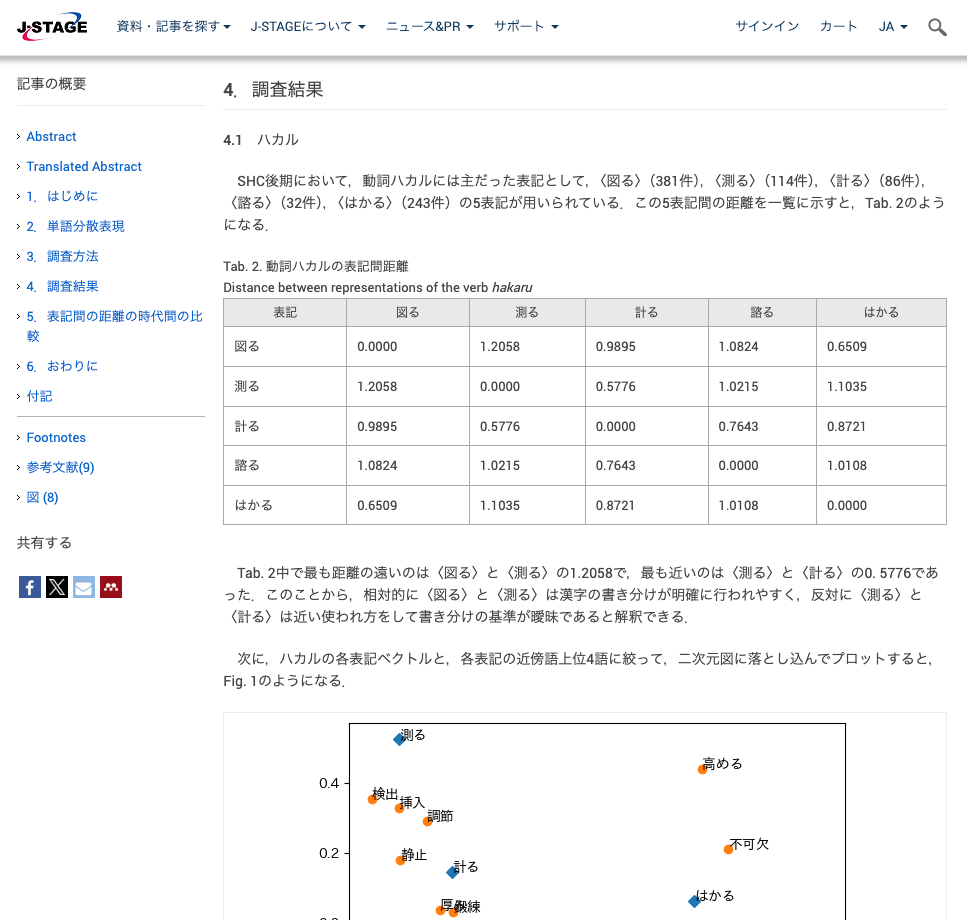
\includegraphics[height=0.80\textheight]{./img/ja_paper_web_2.png}\end{center}
        \end{overprint}
    \end{figure}
\end{frame}

\begin{frame}[t]{自己紹介}
    ほげ
\end{frame}

\section{まとめ}

\begin{frame}[t]{ご清聴ありがとうございました}
    tarek（タレク）\\
    株式会社Helpfeel
    \begin{columns}
    \begin{column}{0.3\textwidth}
        \begin{center}
        \begin{figure}
        
\includegraphics[width=0.7\textwidth]{./img/qr_github.png}
        \end{figure}
        \footnotesize\texttt{github.com/IllDepence}
        \end{center}
    \end{column}
    \begin{column}{0.3\textwidth}
        \begin{center}
        \begin{figure}
        
\includegraphics[width=0.7\textwidth]{./img/qr_blog.png}
        \end{figure}
        \footnotesize\texttt{sirtetris.com}
        \end{center}
    \end{column}
    \begin{column}{0.3\textwidth}
        \begin{center}
        \begin{figure}
        
\includegraphics[width=0.7\textwidth]{./img/qr_slides.png}
        \end{figure}
        \footnotesize\texttt{スライド}
        \end{center}
    \end{column}
    \end{columns}
\end{frame}

\end{document}
